\documentclass[11pt]{article}

\usepackage[utf8]{inputenc}
\usepackage[T1]{fontenc}
\usepackage[margin=2.5cm]{geometry}
\usepackage{amsmath}
\usepackage{amssymb}
\usepackage{booktabs}
\usepackage{array}
\usepackage{tikz}
\usetikzlibrary{arrows.meta}
\usepackage[hidelinks]{hyperref}

\newcommand{\first}{\textsc{First}}
\newcommand{\follow}{\textsc{Follow}}
\newcommand{\closure}{\textsc{Closure}}
\newcommand{\gotofn}{\textsc{Goto}}

\title{Formal Languages --- Final Project\\[2mm]
\large \first{} and \follow{} sets, $LL(1)$ and $SLR(1)$ parsers,\\
and a syntax-directed definition}

\author{Juan Manuel Zuluaga \and Santiago Arboleda Giraldo \and Nicol\'as Pati\~no Palacio}

\date{\today}

\begin{document}

\maketitle

\begin{abstract}
\noindent
This report describes our implementation of the final project. We implemented, in
Python~3 and without any parser generator or parsing library, the computation of the
\first{} and \follow{} sets of a context-free grammar, the table-driven $LL(1)$ parser,
the $SLR(1)$ parser built from the canonical collection of $LR(0)$ item sets, and a
generic evaluator of syntax-directed definitions that works with the dependency graph
and a topological order. Every algorithm follows Aho et al., \emph{Compilers:
Principles, Techniques, and Tools} (2nd edition); the section, algorithm or figure that
each part follows is stated below and is repeated in the docstring of the corresponding
module.
\end{abstract}

\tableofcontents

\section{What of the book we followed, and with which data structures}

\subsection{Sections and algorithms}

Table~\ref{tab:sections} lists, part by part, what we read and implemented.

\begin{table}[h]
\centering
\small
\begin{tabular}{@{}llp{7.4cm}@{}}
\toprule
\textbf{Part} & \textbf{File} & \textbf{Section / algorithm of the book} \\
\midrule
\first{} and \follow{}      & \texttt{sets.py}      & Section 4.4.2. The three rules for \first{}$(X)$, the extension of \first{} to a string $X_1X_2\cdots X_n$, and the three rules for \follow{}$(A)$. Both are computed by iteration until nothing changes. \\
\addlinespace
$LL(1)$ condition           & \texttt{ll1.py}       & The condition stated at the beginning of Section 4.4.3, tested on every pair of alternatives of every nonterminal. \\
\addlinespace
Predictive parsing table    & \texttt{ll1.py}       & Algorithm 4.31 (Section 4.4.3), Figure 4.17 for the shape of the table. \\
\addlinespace
$LL(1)$ parser              & \texttt{ll1.py}       & Algorithm 4.34, the table-driven predictive parser of Section 4.4.4 (Figure 4.19), with the trace in the format of Figure 4.21. \\
\addlinespace
$LR(0)$ items               & \texttt{slr1.py}      & Section 4.6.2: \closure{}$(I)$ and \gotofn{}$(I,X)$ of Figure 4.32, and the canonical collection of Figure 4.33, on the augmented grammar $S' \rightarrow S$. \\
\addlinespace
$SLR(1)$ tables             & \texttt{slr1.py}      & Algorithm 4.46 (Section 4.6.4), which uses \follow{}. The grammar is $SLR(1)$ iff no cell of \textsc{Action} receives two different entries (Section 4.5.4 for the kinds of conflict). \\
\addlinespace
$SLR(1)$ parser             & \texttt{slr1.py}      & Algorithm 4.44, the $LR$ parsing algorithm of Section 4.6.3 (Figure 4.36), with the trace in the format of Figure 4.38. \\
\addlinespace
SDD                         & \texttt{sdd.py}       & Section 5.1.1 (synthesized and inherited attributes) and the format of Figure 5.1 for the semantic rules. \\
\addlinespace
Evaluation                  & \texttt{evaluator.py} & Section 5.2.1 (dependency graph) and Section 5.2.2 (evaluation order as a topological sort; a cycle means the SDD is circular). The classification uses Sections 5.2.3 and 5.2.4. \\
\bottomrule
\end{tabular}
\caption{Parts of the project and the place in the book that each one follows.}
\label{tab:sections}
\end{table}

\subsection{Data structures}

\begin{itemize}
  \item \textbf{Grammar.} A list of pairs \texttt{(head, body)}, where the body is a
        tuple of one-character symbols and the empty tuple \texttt{()} represents
        $\varepsilon$. The position in that list is the \emph{number} of the production
        and is what the two tables store, so a table entry costs one integer. A
        dictionary \texttt{head $\rightarrow$ list of indices} gives the alternatives of
        a nonterminal without scanning the list.

  \item \textbf{\first{} and \follow{}.} Dictionaries \texttt{symbol $\rightarrow$ set of
        terminals}. $\varepsilon$ is stored inside the set as the string \texttt{e} and
        the end marker as \texttt{\$}, exactly as in the notation of the assignment, so
        printing them is immediate. Using sets makes the fixed-point loop easy to write:
        we repeat the rules until no set changes size.

  \item \textbf{$LL(1)$ table.} A dictionary \texttt{(A, a) $\rightarrow$ list of
        production numbers}. The value is a \emph{list} and not a single number on
        purpose: a cell with more than one element is a conflict, which is how the table
        detects that the grammar is not $LL(1)$.

  \item \textbf{$LR(0)$ items and states.} An item is the pair
        \texttt{(production number, position of the dot)}. A state is the
        \texttt{frozenset} of its items, so two states with the same items are
        automatically the same state and can be used as dictionary keys. The canonical
        collection is a list of those frozensets and \gotofn{} is a dictionary
        \texttt{(state, symbol) $\rightarrow$ state}.

  \item \textbf{\textsc{Action} table.} A dictionary
        \texttt{(state, terminal) $\rightarrow$ (kind, value)} with kind in
        \texttt{\{shift, reduce, accept\}}. Writing an entry over a different one is
        what we record as a conflict.

  \item \textbf{Parse tree.} A node stores its symbol, the number of the production used
        (only for nonterminals), its children and a dictionary of attribute values. Both
        parsers build the same kind of tree, so Item~3 works with either of them.

  \item \textbf{Dependency graph.} An attribute instance is the pair
        \texttt{(number of the node, name of the attribute)}; the nodes are numbered in
        preorder before building the graph so that two nodes with the same symbol are
        never confused. The graph itself is a set of edges, and the topological sort is
        Kahn's algorithm over a counter of incoming edges.
\end{itemize}

\section{Items 1 and 2}

\subsection{The grammar we used}

The grammar below is ours; it is not one of the examples of the assignment. It describes
a block that contains a list of items, where an item is either an identifier
\texttt{i} or another block. It is recursive, it has an $\varepsilon$-production, and it
is both $LL(1)$ and $SLR(1)$, so both parsers can be shown on it.

\begin{center}
\small
\begin{verbatim}
3
S -> {L}
L -> IL e
I -> {L} i
\end{verbatim}
\end{center}

In the notation of the book:
\[
S \rightarrow \texttt{\{}\,L\,\texttt{\}}
\qquad
L \rightarrow I\,L \mid \varepsilon
\qquad
I \rightarrow \texttt{\{}\,L\,\texttt{\}} \mid \texttt{i}
\]

\subsection{\first{} and \follow{} (Item 1)}

Output of \texttt{python main.py -\,-sets} on that grammar:

\begin{center}
\small
\begin{verbatim}
First(I) = {i, {}
First(L) = {i, {, e}
First(S) = {{}
Follow(I) = {i, {, }}
Follow(L) = {}}
Follow(S) = {$}
\end{verbatim}
\end{center}

Note how $\varepsilon$ is handled: $L$ has the production $L \rightarrow \varepsilon$, so
\texttt{e} belongs to \first{}$(L)$. Because $L$ is nullable, in $L \rightarrow IL$ the
symbol $I$ is followed by $\first{}(L)\setminus\{\varepsilon\}=\{\texttt{i},\texttt{\{}\}$
(rule~2) and, since $L$ can disappear, also by everything in \follow{}$(L)$ (rule~3). That
is why $\follow{}(I)=\{\texttt{i},\texttt{\{},\texttt{\}}\}$. In turn,
$\follow{}(L)=\{\texttt{\}}\}$ comes from rule~2 applied to $S \rightarrow \texttt{\{}L\texttt{\}}$
and to $I \rightarrow \texttt{\{}L\texttt{\}}$, where $L$ is always followed by \texttt{\}}.
The end marker \texttt{\$} appears only in \follow{}$(S)$, by rule~1.

\subsection{Predictive parsing table (Algorithm 4.31)}

\begin{center}
\small
\begin{verbatim}
        i         {         }         $
I     I -> i   I -> {L}
L    L -> IL   L -> IL    L -> e
S              S -> {L}
\end{verbatim}
\end{center}

No cell holds two productions, and the pairwise test of Section 4.4.3 passes as well:
for $I$, \first{}$(\texttt{\{}L\texttt{\}}) = \{\texttt{\{}\}$ and
\first{}$(\texttt{i}) = \{\texttt{i}\}$ are disjoint; for $L$,
\first{}$(IL) = \{\texttt{i},\texttt{\{}\}$ does not meet
\follow{}$(L) = \{\texttt{\}}\}$, which is the condition that the $\varepsilon$
alternative has to satisfy. The grammar is therefore $LL(1)$.

\subsection{Canonical collection of $LR(0)$ item sets (Section 4.6.2)}

The grammar is augmented with $S' \rightarrow S$. The collection our program computes
has eleven states:

\begin{center}
\scriptsize
\begin{verbatim}
I0:                      I4:                      I8:
    S' -> .S                 S -> {L.}                S -> {L}.
    S -> .{L}                GOTO(I4, }) = I8
    GOTO(I0, S) = I1                              I9:
    GOTO(I0, {) = I2     I5:                          I -> {L.}
                             I -> i.                  GOTO(I9, }) = I10
I1:
    S' -> S.             I6:                      I10:
                             L -> .IL                 I -> {L}.
I2:                          L -> .
    S -> {.L}                I -> .{L}
    L -> .IL                 I -> {.L}
    L -> .                   I -> .i
    I -> .{L}                GOTO(I6, I) = I3
    I -> .i                  GOTO(I6, L) = I9
    GOTO(I2, I) = I3         GOTO(I6, i) = I5
    GOTO(I2, L) = I4         GOTO(I6, {) = I6
    GOTO(I2, i) = I5
    GOTO(I2, {) = I6     I7:
                             L -> IL.
I3:
    L -> .IL
    L -> I.L
    L -> .
    I -> .{L}
    I -> .i
    GOTO(I3, I) = I3
    GOTO(I3, L) = I7
    GOTO(I3, i) = I5
    GOTO(I3, {) = I6
\end{verbatim}
\end{center}

\subsection{\textsc{Action} and \gotofn{} tables (Algorithm 4.46)}

\begin{center}
\small
\begin{verbatim}
Numbered productions:
    1. S -> {L}
    2. L -> IL
    3. L -> e
    4. I -> {L}
    5. I -> i

STATE    i     {     }     $    |  I     L     S
0              s2               |              1
1                         acc   |
2        s5    s6    r3         |  3     4
3        s5    s6    r3         |  3     7
4                    s8         |
5        r5    r5    r5         |
6        s5    s6    r3         |  3     9
7                    r2         |
8                          r1   |
9                   s10         |
10       r4    r4    r4         |
\end{verbatim}
\end{center}

States 2, 3 and 6 are the interesting ones: they contain the complete item
$L \rightarrow \;\cdot$ and also items with the dot before a terminal. There is no
shift/reduce conflict because the reduction $L \rightarrow \varepsilon$ is written only
in the columns of \follow{}$(L) = \{\texttt{\}}\}$, while the shifts are on \texttt{i}
and \texttt{\{}. This is exactly the difference between an $LR(0)$ and an $SLR(1)$
table. No cell has two entries, so the grammar is $SLR(1)$.

\subsection{A string parsed step by step}

We parse \texttt{\{i\{i\}\}} with both parsers. With the $LL(1)$ parser (format of
Figure 4.21; the stack is written bottom-to-top):

\begin{center}
\small
\begin{verbatim}
STACK                   INPUT           ACTION
$S                      {i{i}}$         output S -> {L}
$}L{                    {i{i}}$         match {
$}L                     i{i}}$          output L -> IL
$}LI                    i{i}}$          output I -> i
$}Li                    i{i}}$          match i
$}L                     {i}}$           output L -> IL
$}LI                    {i}}$           output I -> {L}
$}L}L{                  {i}}$           match {
$}L}L                   i}}$            output L -> IL
$}L}LI                  i}}$            output I -> i
$}L}Li                  i}}$            match i
$}L}L                   }}$             output L -> e
$}L}                    }}$             match }
$}L                     }$              output L -> e
$}                      }$              match }
$                       $               accept
\end{verbatim}
\end{center}

With the $SLR(1)$ parser (format of Figure 4.38):

\begin{center}
\small
\begin{verbatim}
STACK                 SYMBOLS       INPUT         ACTION
0                                   {i{i}}$       shift 2
0 2                   {             i{i}}$        shift 5
0 2 5                 {i            {i}}$         reduce I -> i
0 2 3                 {I            {i}}$         shift 6
0 2 3 6               {I{           i}}$          shift 5
0 2 3 6 5             {I{i          }}$           reduce I -> i
0 2 3 6 3             {I{I          }}$           reduce L -> e
0 2 3 6 3 7           {I{IL         }}$           reduce L -> IL
0 2 3 6 9             {I{L          }}$           shift 10
0 2 3 6 9 10          {I{L}         }$            reduce I -> {L}
0 2 3 3               {II           }$            reduce L -> e
0 2 3 3 7             {IIL          }$            reduce L -> IL
0 2 3 7               {IL           }$            reduce L -> IL
0 2 4                 {L            }$            shift 8
0 2 4 8               {L}           $             reduce S -> {L}
0 1                   S             $             accept
\end{verbatim}
\end{center}

The two parsers accept the same strings, which is what one expects: the top-down parser
produces the leftmost derivation from the root down, and the bottom-up parser produces
the reverse of a rightmost derivation.

\section{Item 3: the syntax-directed definition}

\subsection{Step 1: the grammar}

\begin{center}
\small
\begin{verbatim}
5
S -> N#B
N -> DR
R -> DR e
D -> 0 1 2
B -> b t
\end{verbatim}
\end{center}

A string of this language is a sequence of digits, then \texttt{\#}, then one letter that
says in which base the digits must be read: \texttt{b} for base 2 and \texttt{t} for base
3. For instance \texttt{102\#t} is the numeral $102$ in base 3, which is $11$, and
\texttt{1011\#b} is $1011$ in base 2, which is also $11$.

The grammar satisfies the three conditions of Step 1:

\begin{itemize}
  \item[\textbf{G1}] It follows the conventions of Section 2.2 and our own program
        reports that it is \emph{both} $LL(1)$ and $SLR(1)$, so the strings are parsed
        with the parsers of Item~2. (The evaluator accepts either one; the tests check
        that both give the same values.)
  \item[\textbf{G2}] It has five nonterminals and nine productions, and $R$ is
        recursive.
  \item[\textbf{G3}] Neither the grammar nor the SDD is in the book or in the
        assignment. The idea of accumulating a value from left to right is taken from the
        book, but the computation is different: here the \emph{base} is not fixed, it is
        read at the end of the string and travels back to the first digit.
\end{itemize}

\subsection{Step 2.1: the attributes}

\begin{table}[h]
\centering
\small
\begin{tabular}{@{}llllp{6.2cm}@{}}
\toprule
\textbf{Symbol} & \textbf{Attribute} & \textbf{Kind} & \textbf{Type} & \textbf{Meaning} \\
\midrule
$S$ & \textit{val}    & synthesized & integer   & value of the whole numeral \\
$N$ & \textit{base}   & inherited   & integer   & base in which the digits must be read \\
$N$ & \textit{acc}    & inherited   & integer   & value accumulated before the first digit \\
$N$ & \textit{val}    & synthesized & integer   & value of the whole list of digits \\
$R$ & \textit{base}   & inherited   & integer   & base in which the digits must be read \\
$R$ & \textit{acc}    & inherited   & integer   & value of the digits already read \\
$R$ & \textit{val}    & synthesized & integer   & accumulated value when the list ends \\
$D$ & \textit{val}    & synthesized & integer   & value of the digit \\
$B$ & \textit{val}    & synthesized & integer   & base named by the final letter \\
terminal & \textit{lexval} & synthesized & character & the character itself \\
\bottomrule
\end{tabular}
\caption{Attributes of the SDD. Terminals only have the synthesized attribute
\textit{lexval}, which the parser already knows, so no scanner is needed.}
\label{tab:attributes}
\end{table}

There are three different attributes, \textit{val} (synthesized), \textit{base} and
\textit{acc} (both inherited), and the start symbol $S$ has no inherited attribute, as
the assignment requires.

\subsection{Step 2.2: the semantic rules}

\begin{table}[h]
\centering
\small
\begin{tabular}{@{}ll@{}}
\toprule
\textbf{Production} & \textbf{Semantic rules} \\
\midrule
$S \rightarrow N\,\texttt{\#}\,B$ & $N.base = B.val;\quad N.acc = 0;\quad S.val = N.val$ \\
\addlinespace
$N \rightarrow D\,R$ & $R.base = N.base;\quad R.acc = N.acc \times N.base + D.val;$ \\
                     & $N.val = R.val$ \\
\addlinespace
$R \rightarrow D\,R_1$ & $R_1.base = R.base;\quad R_1.acc = R.acc \times R.base + D.val;$ \\
                       & $R.val = R_1.val$ \\
\addlinespace
$R \rightarrow \varepsilon$ & $R.val = R.acc$ \\
\addlinespace
$D \rightarrow \texttt{0}$ & $D.val = \textit{digit}(\texttt{0}.lexval)$ \\
$D \rightarrow \texttt{1}$ & $D.val = \textit{digit}(\texttt{1}.lexval)$ \\
$D \rightarrow \texttt{2}$ & $D.val = \textit{digit}(\texttt{2}.lexval)$ \\
\addlinespace
$B \rightarrow \texttt{b}$ & $B.val = \textit{base}(\texttt{b}.lexval) = 2$ \\
$B \rightarrow \texttt{t}$ & $B.val = \textit{base}(\texttt{t}.lexval) = 3$ \\
\bottomrule
\end{tabular}
\caption{The SDD, in the format of Figure 5.1 of the book.}
\label{tab:sdd}
\end{table}

The two checks of Section 5.1.1 hold for every production:

\begin{itemize}
  \item Every rule defines either a synthesized attribute of the head or an inherited
        attribute of a symbol of the body, and uses only attributes of symbols of that
        same production.
  \item In every production, each synthesized attribute of the head and each inherited
        attribute of each nonterminal of the body is defined exactly once. In
        $S \rightarrow N\texttt{\#}B$, for example, $S.val$ is defined once and the two
        inherited attributes of $N$ are defined once each; $B$ has no inherited
        attributes, so there is nothing to define for it.
\end{itemize}

\subsection{Step 3: an example by hand}

We take the string \texttt{102\#t}, which has five terminals. Its parse tree, annotated
with the value of every attribute, is shown in Figure~\ref{fig:tree}. The number in
brackets is the number our program gives to the node (preorder), and it is used to name
the attribute instances in the dependency graph.

\begin{figure}[h]
\centering
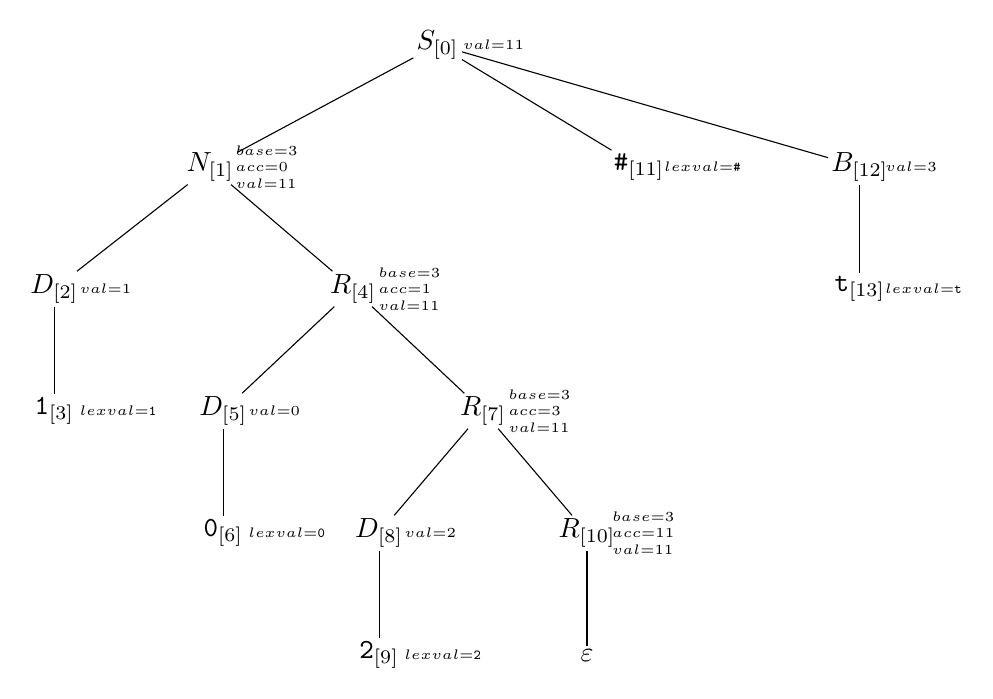
\begin{tikzpicture}[x=1.65cm, y=1.55cm, every node/.style={inner sep=1pt}]

\node (S)  at (3.25, 0)  {$S_{[0]}$};
\node (N)  at (1.50,-1)  {$N_{[1]}$};
\node (H)  at (4.80,-1)  {$\texttt{\#}_{[11]}$};
\node (B)  at (6.50,-1)  {$B_{[12]}$};
\node (D2) at (0.30,-2)  {$D_{[2]}$};
\node (R4) at (2.60,-2)  {$R_{[4]}$};
\node (T)  at (6.50,-2)  {$\texttt{t}_{[13]}$};
\node (L3) at (0.30,-3)  {$\texttt{1}_{[3]}$};
\node (D5) at (1.60,-3)  {$D_{[5]}$};
\node (R7) at (3.60,-3)  {$R_{[7]}$};
\node (L6) at (1.60,-4)  {$\texttt{0}_{[6]}$};
\node (D8) at (2.80,-4)  {$D_{[8]}$};
\node (R10)at (4.40,-4)  {$R_{[10]}$};
\node (L9) at (2.80,-5)  {$\texttt{2}_{[9]}$};
\node (EP) at (4.40,-5)  {$\varepsilon$};

\draw (S)--(N); \draw (S)--(H); \draw (S)--(B);
\draw (N)--(D2); \draw (N)--(R4);
\draw (B)--(T);
\draw (D2)--(L3);
\draw (R4)--(D5); \draw (R4)--(R7);
\draw (D5)--(L6);
\draw (R7)--(D8); \draw (R7)--(R10);
\draw (D8)--(L9);
\draw (R10)--(EP);

\node[anchor=west, align=left, font=\tiny] at (3.42, 0)  {$val{=}11$};
\node[anchor=west, align=left, font=\tiny] at (1.67,-1)  {$base{=}3$\\$acc{=}0$\\$val{=}11$};
\node[anchor=west, align=left, font=\tiny] at (4.97,-1)  {$lexval{=}\texttt{\#}$};
\node[anchor=west, align=left, font=\tiny] at (6.67,-1)  {$val{=}3$};
\node[anchor=west, align=left, font=\tiny] at (0.47,-2)  {$val{=}1$};
\node[anchor=west, align=left, font=\tiny] at (2.77,-2)  {$base{=}3$\\$acc{=}1$\\$val{=}11$};
\node[anchor=west, align=left, font=\tiny] at (6.67,-2)  {$lexval{=}\texttt{t}$};
\node[anchor=west, align=left, font=\tiny] at (0.47,-3)  {$lexval{=}\texttt{1}$};
\node[anchor=west, align=left, font=\tiny] at (1.77,-3)  {$val{=}0$};
\node[anchor=west, align=left, font=\tiny] at (3.77,-3)  {$base{=}3$\\$acc{=}3$\\$val{=}11$};
\node[anchor=west, align=left, font=\tiny] at (1.77,-4)  {$lexval{=}\texttt{0}$};
\node[anchor=west, align=left, font=\tiny] at (2.97,-4)  {$val{=}2$};
\node[anchor=west, align=left, font=\tiny] at (4.57,-4)  {$base{=}3$\\$acc{=}11$\\$val{=}11$};
\node[anchor=west, align=left, font=\tiny] at (2.97,-5)  {$lexval{=}\texttt{2}$};

\end{tikzpicture}
\caption{Annotated parse tree of \texttt{102\#t}. The value of the main attribute is
$S.val = 11$, because $1\cdot 3^2 + 0 \cdot 3 + 2 = 11$.}
\label{fig:tree}
\end{figure}

The dependency graph (Section 5.2.1) is shown in Figure~\ref{fig:graph}. There is one
vertex per attribute of each node and one edge from every attribute that a rule uses to
the attribute that the rule defines. The vertices are drawn by levels, so that every
edge goes downwards.

\begin{figure}[h]
\centering
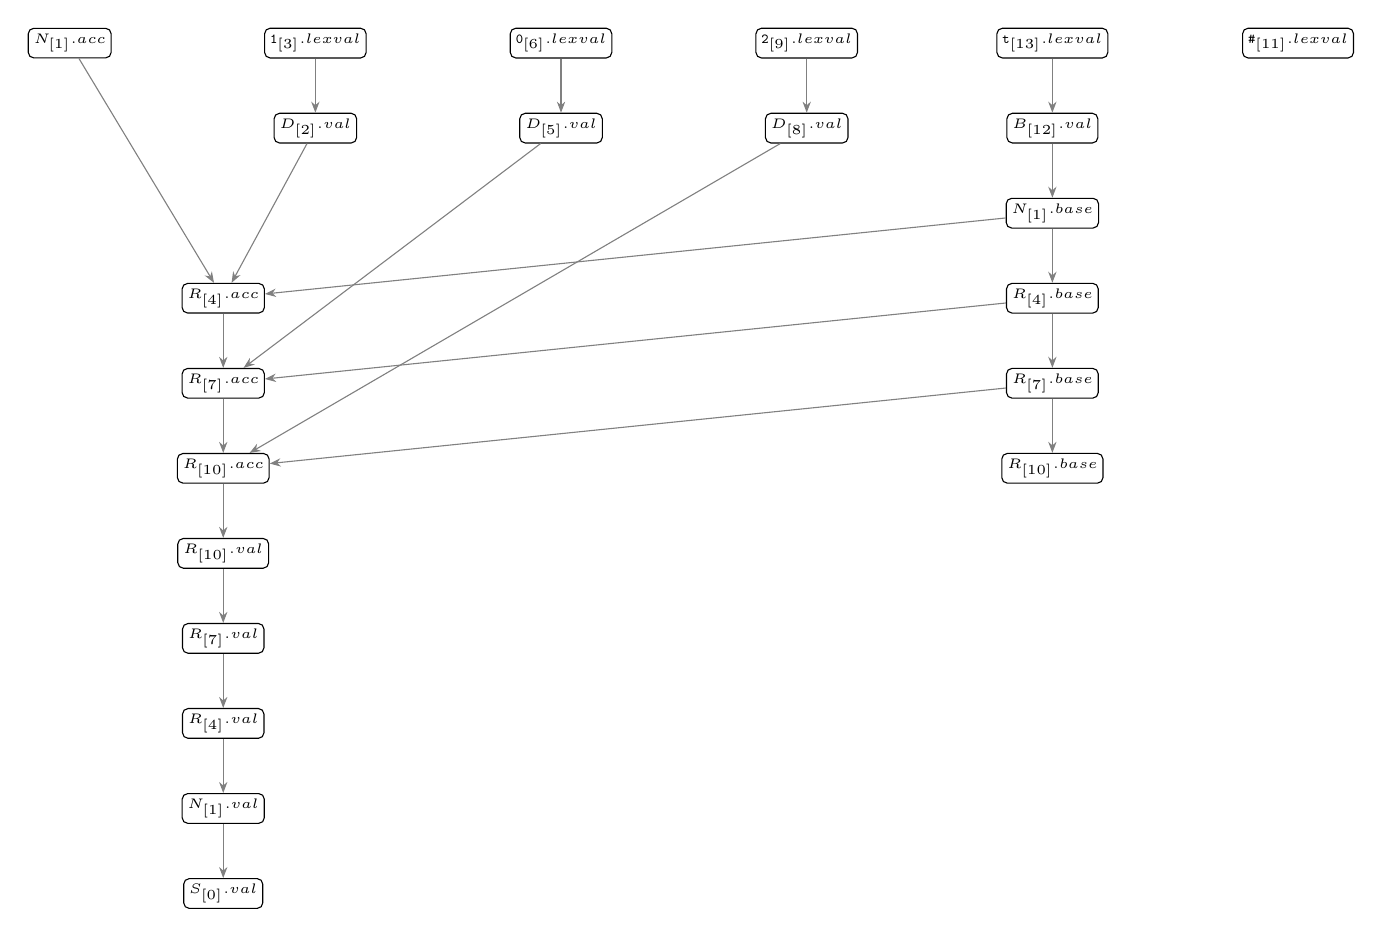
\begin{tikzpicture}[
  x=1.95cm, y=1.08cm,
  v/.style={draw, rounded corners=2pt, inner sep=2pt, font=\tiny, fill=white},
  e/.style={-{Stealth[length=4pt]}, gray}
]

\node[v] (nacc)   at (0.0, 0)  {$N_{[1]}.acc$};
\node[v] (l3)     at (1.6, 0)  {$\texttt{1}_{[3]}.lexval$};
\node[v] (l6)     at (3.2, 0)  {$\texttt{0}_{[6]}.lexval$};
\node[v] (l9)     at (4.8, 0)  {$\texttt{2}_{[9]}.lexval$};
\node[v] (l13)    at (6.4, 0)  {$\texttt{t}_{[13]}.lexval$};
\node[v] (l11)    at (8.0, 0)  {$\texttt{\#}_{[11]}.lexval$};

\node[v] (d2)     at (1.6,-1)  {$D_{[2]}.val$};
\node[v] (d5)     at (3.2,-1)  {$D_{[5]}.val$};
\node[v] (d8)     at (4.8,-1)  {$D_{[8]}.val$};
\node[v] (b12)    at (6.4,-1)  {$B_{[12]}.val$};

\node[v] (nbase)  at (6.4,-2)  {$N_{[1]}.base$};

\node[v] (r4acc)  at (1.0,-3)  {$R_{[4]}.acc$};
\node[v] (r4base) at (6.4,-3)  {$R_{[4]}.base$};
\node[v] (r7acc)  at (1.0,-4)  {$R_{[7]}.acc$};
\node[v] (r7base) at (6.4,-4)  {$R_{[7]}.base$};
\node[v] (r10acc) at (1.0,-5)  {$R_{[10]}.acc$};
\node[v] (r10base)at (6.4,-5)  {$R_{[10]}.base$};

\node[v] (r10val) at (1.0,-6)  {$R_{[10]}.val$};
\node[v] (r7val)  at (1.0,-7)  {$R_{[7]}.val$};
\node[v] (r4val)  at (1.0,-8)  {$R_{[4]}.val$};
\node[v] (nval)   at (1.0,-9)  {$N_{[1]}.val$};
\node[v] (sval)   at (1.0,-10) {$S_{[0]}.val$};

\draw[e] (l3)  -- (d2);
\draw[e] (l6)  -- (d5);
\draw[e] (l9)  -- (d8);
\draw[e] (l13) -- (b12);
\draw[e] (b12) -- (nbase);

\draw[e] (nacc)  -- (r4acc);
\draw[e] (nbase) -- (r4acc);
\draw[e] (d2)    -- (r4acc);
\draw[e] (nbase) -- (r4base);

\draw[e] (r4acc)  -- (r7acc);
\draw[e] (r4base) -- (r7acc);
\draw[e] (d5)     -- (r7acc);
\draw[e] (r4base) -- (r7base);

\draw[e] (r7acc)  -- (r10acc);
\draw[e] (r7base) -- (r10acc);
\draw[e] (d8)     -- (r10acc);
\draw[e] (r7base) -- (r10base);

\draw[e] (r10acc) -- (r10val);
\draw[e] (r10val) -- (r7val);
\draw[e] (r7val)  -- (r4val);
\draw[e] (r4val)  -- (nval);
\draw[e] (nval)   -- (sval);

\end{tikzpicture}
\caption{Dependency graph of \texttt{102\#t}. The vertex
$\texttt{\#}_{[11]}.lexval$ is isolated: the semantic rules never use it. The vertex
$R_{[10]}.base$ is defined but never used either, because $R_{[10]}$ applies
$R \rightarrow \varepsilon$.}
\label{fig:graph}
\end{figure}

A valid evaluation order is any topological order of that graph. The one our program
produces is the following (it is the order printed by \texttt{sdd\_main.py}):

\begin{center}
\small
\begin{verbatim}
  1. N[1].acc     = 0          12. R[4].acc    = 1
  2. 1[3].lexval  = '1'        13. R[4].base   = 3
  3. D[2].val     = 1          14. R[7].acc    = 3
  4. 0[6].lexval  = '0'        15. R[7].base   = 3
  5. D[5].val     = 0          16. R[10].acc   = 11
  6. 2[9].lexval  = '2'        17. R[10].base  = 3
  7. D[8].val     = 2          18. R[10].val   = 11
  8. #[11].lexval = '#'        19. R[7].val    = 11
  9. t[13].lexval = 't'        20. R[4].val    = 11
 10. B[12].val    = 3          21. N[1].val    = 11
 11. N[1].base    = 3          22. S[0].val    = 11
\end{verbatim}
\end{center}

The important step is number 11: $N_{[1]}.base$ can only be computed after
$B_{[12]}.val$, which belongs to a node that is \emph{to the right} of $N$ in the tree.
Everything that accumulates the digits has to wait for it.

\subsection{Step 4: classification of the SDD}

Our SDD is \textbf{neither $S$-attributed nor $L$-attributed}.

\begin{itemize}
  \item It is not $S$-attributed (Section 5.2.3): an $S$-attributed SDD has only
        synthesized attributes, and ours has the inherited attributes
        $N.base$, $N.acc$, $R.base$ and $R.acc$.

  \item It is not $L$-attributed (Section 5.2.4). The definition requires that, in a
        production $A \rightarrow X_1 X_2 \cdots X_n$, every inherited attribute of
        $X_i$ depend only on inherited attributes of $A$, on attributes of
        $X_1,\dots,X_{i-1}$, or on attributes of $X_i$ itself in a non-circular way. In
        the production
        \[
          S \rightarrow \underbrace{N}_{X_1}\ \underbrace{\texttt{\#}}_{X_2}\ \underbrace{B}_{X_3},
          \qquad N.base = B.val,
        \]
        the inherited attribute of $X_1$ depends on an attribute of $X_3$, which is to
        its right. That is exactly what an $L$-attributed definition forbids. All the
        other productions do satisfy the condition, but one counterexample is enough.
\end{itemize}

This was deliberate. An $L$-attributed SDD can be evaluated with a single recursive
pass over the tree that visits the children from left to right, so the general method
would never be exercised. Here that pass fails --- when it reaches $N$ it does not yet
know the base --- while the dependency graph and the topological order work without any
change, which is the point of the method of Section 5.2.2. The SDD is still
non-circular, so a valid evaluation order always exists.

\subsection{Step 5: the implementation}

The implementation follows the five points of Step 5 of the assignment.

\begin{enumerate}
  \item \textbf{The SDD is data, not code.} The file \texttt{sdd.py} holds a dictionary
        that maps every production to its list of semantic rules, and each rule stores
        the attribute it defines, the list of attributes it uses, and the function that
        computes it. Attributes are referred to by \emph{position} inside the
        production: $0$ is the head, $1$ is the first symbol of the body, and so on.
        The rule $R.acc = N.acc \times N.base + D.val$, for instance, is stored as the
        target $(2,\textit{acc})$, the dependencies
        $[(0,\textit{acc}), (0,\textit{base}), (1,\textit{val})]$ and the function
        \verb|lambda v: v[0]*v[1] + v[2]|.

  \item \textbf{Parse tree.} The string is parsed with the $LL(1)$ parser of Item~2 (or
        with the $SLR(1)$ one, with the flag \texttt{-\,-slr}), and the parser builds the
        tree as it works: the top-down parser creates the children when it expands a
        nonterminal, and the bottom-up parser pops $|\beta|$ nodes and makes them the
        children of the new node when it reduces by $A \rightarrow \beta$.

  \item \textbf{Dependency graph.} \texttt{evaluator.py} walks the tree, and for every
        internal node it looks up the rules of its production and instantiates them: the
        positions are replaced by the actual nodes, and for every dependency an edge is
        added from the attribute that is used to the attribute that is defined. Leaves
        contribute their \textit{lexval}, which the parser already filled in.

  \item \textbf{Order and evaluation.} Kahn's algorithm gives a topological order; among
        the vertices that are ready we always take the smallest one, so that the output
        is the same in every run. If some vertex never becomes ready, the graph has a
        cycle, and the program reports that the SDD is circular and stops without
        evaluating anything. Otherwise the attributes are computed in that order.

  \item \textbf{Output.} For every string the program prints \texttt{no}, or the
        annotated tree (one node per line, indented by depth), the evaluation order and
        the value of the main attribute $S.val$.
\end{enumerate}

\texttt{evaluator.py} never mentions \textit{base}, \textit{acc} or \textit{val}:
replacing the dictionary of \texttt{sdd.py} is enough to evaluate a completely different
SDD, which is what the assignment asks for.

\subsection{Step 6: tests}

Table~\ref{tab:tests} shows the strings we used. They include the shortest string of the
language, a string that is not in the language, and a string with deep recursion. All of
them are also in the automatic test suite (\texttt{python tests.py}).

\begin{table}[h]
\centering
\small
\begin{tabular}{@{}lll@{}}
\toprule
\textbf{String} & \textbf{Result} & \textbf{Why} \\
\midrule
\texttt{0\#b}       & $S.val = 0$   & shortest string of the language (one digit) \\
\texttt{102\#t}     & $S.val = 11$  & the example worked out by hand \\
\texttt{1011\#b}    & $S.val = 11$  & the same value written in base 2 \\
\texttt{210201\#t}  & $S.val = 586$ & six digits, so the recursion on $R$ is six levels deep \\
\texttt{102}        & \texttt{no}   & the base is missing \\
\texttt{121\#x}     & \texttt{no}   & \texttt{x} is not a terminal of the grammar \\
\texttt{e} (empty)  & \texttt{no}   & the language has no empty string \\
\bottomrule
\end{tabular}
\caption{Test strings and their results.}
\label{tab:tests}
\end{table}

\paragraph{Circular SDD.} To show that the evaluator detects circularity, we changed one
rule of the production $R \rightarrow D\,R_1$: instead of
$R_1.acc = R.acc \times R.base + D.val$ we wrote $R_1.acc = R.val$. Since
$R.val = R_1.val$ and $R_1.val$ ends up depending on $R_1.acc$, the graph gets the cycle
\[
  R.val \;\rightarrow\; R_1.acc \;\rightarrow\; R_1.val \;\rightarrow\; R.val .
\]
That version is kept in \texttt{sdd.py} as \texttt{CIRCULAR\_SDD} and is used with the
flag \texttt{-\,-circular}. Running \verb|python sdd_main.py --circular| on
\texttt{102\#t} prints:

\begin{center}
\small
\begin{verbatim}
Cadena: 102#t
La SDD es circular: el grafo de dependencias tiene un ciclo.
Atributos que quedaron sin poder evaluarse:
    S[0].val
    N[1].val
    R[4].val
    R[7].acc
    R[7].val
    R[10].acc
    R[10].val
\end{verbatim}
\end{center}

On the string \texttt{0\#b} the same circular SDD evaluates normally, because that tree
never uses the production $R \rightarrow D\,R_1$ and therefore never builds the cycle.
Circularity is a property of each particular tree, not of the SDD alone, which matches
what Section 5.2.2 says.

\section{Extra: web interface}

Besides the two console programs, we built a small web application. It does not
implement any algorithm of its own: it calls exactly the same functions, so whatever the
page shows is what \texttt{main.py} and \texttt{sdd\_main.py} print. We kept the layered
architecture we had used in the previous assignment of the course:

\begin{center}
\small
\begin{tabular}{@{}llp{6.6cm}@{}}
\toprule
\textbf{Layer} & \textbf{File} & \textbf{Responsibility} \\
\midrule
\addlinespace
Controller & \texttt{app.py} & Flask routes. Validates the shape of the request and turns results or errors into HTTP responses. \\
\addlinespace
Gateway & \texttt{gateway.py} & Turns the internal structures (sets, frozensets of items, tree nodes) into JSON, and every domain error into a \texttt{GatewayError}. \\
\addlinespace
Algorithms & Items 1--3 & Unchanged. They know nothing about HTTP or Flask. \\
\addlinespace
View & \texttt{analyzer.html} & One page, no external dependencies. \\
\bottomrule
\end{tabular}
\end{center}

The endpoints are \texttt{POST /api/grammar} (sets, tables, $LR(0)$ automaton and
verdict), \texttt{POST /api/parse} (parses strings and returns the trace and the tree),
\texttt{POST /api/sdd} (evaluates the SDD) and \texttt{GET /analyzer} (the page). A
malformed request gets a \texttt{400} and one that the algorithms reject gets a
\texttt{422}, always as JSON.

The page is worth it for two things that are hard to read in a terminal. The parse tree
is drawn as SVG with every node annotated with its attributes, which is the annotated
tree of Figure~\ref{fig:tree} but generated automatically for any string. And the
dependency graph is drawn by levels, with one level per step of the topological order,
so that every edge goes downwards and the shape of the graph is visible at a glance;
when the circular SDD is selected, the attributes that end up inside the cycle are drawn
in red. Making the drawing forced us to be precise about the direction of the edges,
because a graph drawn with the edges reversed looks obviously wrong on screen.

\section{Problems we found, and how we solved them}

\begin{enumerate}
  \item \textbf{\first{} of a string versus \first{} of a symbol.} Our first version
        only computed \first{}$(X)$ for single symbols, and the $LL(1)$ table came out
        wrong for productions whose body starts with a nullable nonterminal. The book
        extends \first{} to strings $X_1\cdots X_n$ in Section 4.4.2 and that extension
        is what Algorithm 4.31 really needs. We wrote it as a separate function
        (\texttt{first\_of\_string}) and the table became correct.

  \item \textbf{Where $\varepsilon$ belongs and where it does not.} $\varepsilon$ can be
        in a \first{} set but never in a \follow{} set. We were adding
        \first{}$(\beta)$ whole to \follow{}$(B)$ in rule 2 instead of
        \first{}$(\beta) \setminus \{\varepsilon\}$, which produced an \texttt{e} inside
        \follow{} and, through Algorithm 4.31, a column that does not exist in the
        table. Writing the two rules with the explicit subtraction fixed it.

  \item \textbf{The temptation to fix the grammar.} The assignment forbids transforming
        the grammar before testing whether it is $LL(1)$. With a left-recursive grammar
        such as $S \rightarrow S{+}T \mid T$, the natural reaction is to remove the left
        recursion so that the $LL(1)$ parser works. We did not: our test simply reports a
        conflict, which is the honest answer, and that grammar is handled by the
        $SLR(1)$ parser (it is Example 1 of the assignment).

  \item \textbf{The offset of the augmented grammar.} In \texttt{slr1.py} production
        number $0$ is $S' \rightarrow S$, so every production of the original grammar is
        shifted by one. We first used those numbers directly when building the parse
        tree and the nodes ended up pointing at the wrong production, which made the SDD
        evaluator complain about rules that did not exist. The fix is one line
        (\verb|production=value - 1|), but finding it took a while because the parser
        kept answering \texttt{yes} correctly; only the tree was wrong.

  \item \textbf{Reproducible output.} Both the canonical collection and the topological
        order depend on the order in which we iterate over sets, and Python does not
        promise a fixed order for sets. Two runs could number the states differently,
        which is confusing when comparing with the book. We iterate over
        \texttt{grammar.symbols()} (a sorted list) when building the collection, and we
        use a heap in the topological sort so that the smallest ready vertex is always
        taken first. Now the output is always the same.

  \item \textbf{Which way the edges go.} The assignment warns about this and we still
        got it wrong the first time: we drew the edge from the attribute that is
        \emph{defined} to the attribute that is \emph{used}. The result was a graph that
        was still acyclic, so nothing crashed --- it simply evaluated the attributes in
        the reverse order and every value came out as \texttt{None}. The rule is the one
        of Section 5.2.1: the edge goes from the attribute that is used to the attribute
        that is defined.

  \item \textbf{Choosing an SDD that is worth the general method.} Our first SDD was
        $L$-attributed, and we realised that a plain recursive traversal evaluated it
        correctly, so the dependency graph was not really doing any work. We changed the
        grammar so that the base appears at the end of the string; now the SDD is neither
        $S$-attributed nor $L$-attributed and the topological order is indispensable.

  \item \textbf{$\varepsilon$-productions in the tree.} A node for
        $A \rightarrow \varepsilon$ has no children, which breaks any code that assumes
        that an internal node has at least one child, and in the $SLR(1)$ parser a
        reduction by an $\varepsilon$-production pops zero states. We decided to keep the
        list of children empty so that the positions of the semantic rules always match
        the body of the production, and to print a line \texttt{e} only when showing the
        tree.
\end{enumerate}

\section{How to run it}

\begin{center}
\small
\begin{verbatim}
python main.py --sets        # Items 1 and 2 (--sets prints FIRST and FOLLOW)
python main.py --tables      # extra: LL(1) table, LR(0) automaton, SLR(1) tables
python main.py --trace       # extra: step-by-step parse of every string
python sdd_main.py           # Item 3
python sdd_main.py --circular    # Item 3 with the circular SDD
python tests.py              # the test suite (67 checks)
python app.py                # extra: web server, page at /analyzer
\end{verbatim}
\end{center}

The \texttt{README.md} file explains the input format and the flags in detail.

\begin{thebibliography}{9}
\bibitem{aho}
Alfred V. Aho, Monica S. Lam, Ravi Sethi and Jeffrey D. Ullman.
\emph{Compilers: Principles, Techniques, and Tools}, 2nd edition.
Addison-Wesley, 2006. ISBN 0321486811.
\end{thebibliography}

\end{document}
